\subsection{System Characterisation}
\label{sec:characterisation}

A systems complete dynamic behaviour around an operating point of interest can
be determined by applying a step function -- $\epsilon(t)$ -- to its input and
recording the system's output. The derivative of the resulting function is the
system's  \textit{impulse  response}  and  can  be  used  to calculate optimal
controller parameters.

Before measuring the step response we first have to select the step amplitude.
If the step amplitude is too small, the plant behaves in an atypical way. This
happens because of small disturbances  which  affect the step response. A good
example for this is static friction. On the  other  hand if the step amplitude
is  too  large,  then  non-linear  effects  will throw off the  accuracy  (and
validity) of the result.

After  a system's  step  response  has  been  measured,  it  is  necessary  to
characterise  and  determine  its  properties before it's possible  to  fit  a
transfer function to it. The method  of  characterisation used here is to find
the point of inflection in the measured step response, through which a tangent
is placed.  The  tangent's  intersection  points  with  the  lower  and  upper
horizontal bounds  are used to determine the dead time $T_u$ and the rise time
$T_g$.  Further, the amplitude $K_s$ of the step response can  be  determined.
This process is illustrated in figure \ref{fig:tu-tg-example}.

\begin{figure}[t]
    \centering
    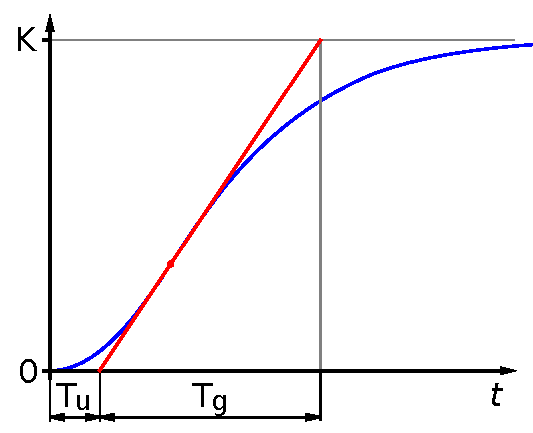
\includegraphics[width=\imagewidth]{images/tu_tg_example}
    \caption{Example step response of a system and measurement of the angle of inflection for determining $K_s$, $T_u$ and $T_g$. Image taken from Wikipedia\cite{ref:tu-tg}.}
    \label{fig:tu-tg-example}
\end{figure}

It is important to note that this method  of  characterisation  is  valid  for
systems with an order of at least $n=2$ and for systems that don't exhibit any
overshoot.

